%!TEX root = ../dissertation.tex
\begin{savequote}[75mm]
Nulla facilisi. In vel sem. Morbi id urna in diam dignissim feugiat. Proin molestie tortor eu velit. Aliquam erat volutpat. Nullam ultrices, diam tempus vulputate egestas, eros pede varius leo.
\qauthor{Quoteauthor Lastname}
\end{savequote}

\chapter{Emerging abstractions: Lexical conventions are shaped by communicative context}
\graphicspath{{./figures/artificial/}}


%% Set up problem
Natural languages provide speakers with remarkable flexibility in the labels they may use to refer to things \cite{Brown58_HowShallAThingBeCalled}. %,Cruse77_PragmaticsLexicalSpecificity
On top of an abundance of expressions made available by syntactic combination and semantic compositionality \cite{Partee95_LexicalSemanticsCompositionality}, we have a number of overlapping and nested terms in our lexicon. \emph{Fido}, \emph{Dalmatian}, \emph{dog}, and \emph{animal} can all reasonably be used to talk about the same entity at different levels of abstraction. How these overlapping meanings are learned, and why speakers choose different levels of specificity in different contexts, is increasingly well-understood \cite<e.g.>{XuTenenbaum07_WordLearningBayesian,GrafEtAl16_BasicLevel} 
but there remains a more fundamental question about the structure of our lexicon: why and how do different levels of abstraction become lexicalized in the first place? %And why do we have words for some abstractions but not for others?

%% Overview of big-picture optimal expressivity theory suggesting an answer
One functional answer is suggested by recent computational approaches to language evolution, which have argued that the lexical conventions of languages balance simplicity, or learnability, with the communicative needs of their users. This optimal expressivity hypothesis accounts well for the lexical distributions found in natural languages across semantic domains like color words and kinship categories \cite{RegierKempKay15_WordMeaningsEfficientCommunication,GibsonEtAl17_ColorNamingUse}, as well as the compositional systems that emerge under iterated learning with communication in the lab \cite{WintersKirbySmith14_LanguagesAdapt, KirbyTamarizCornishSmith15_CompressionCommunication}. A key prediction is that the lexicon of a group should be sensitive to the pragmatic demands of their environment. For example, languages in warm regions ought to be more likely to collapse the distinction between ice and snow into a single word, simply because there are fewer occasions that require distinguishing between the two \cite{RegierCarstensenKemp16_WordsForSnow}. 

%% Limitations of past studies
Still, there are several limitations to the current evidence for this hypothesis. 
First, much of the relevant evidence is observational, aggregated at the level of overall language statistics, not by directly manipulating the contextual conditions of individual language users. 
Second, previous experimental studies have largely focused on the functional outcomes of an iterated learning process, %thus providing a functional argument for when different systems are appropriate. 
but have not grounded the results of this process in a cognitive, mechanistic account of lexical adaptation and convention-formation among individual agents. 
Finally, the phenomenon of reference taxonomies poses a further theoretical challenge: why do languages have hierarchies of terms instead of flatly partitioning the space into category labels as previous work has assumed?

%% Make the case for zooming into dyadic convention formation
While globally shared conventions of a language are shaped over the multi-generational timescales of cultural evolution, contextual pressures operate on the shorter timescales of dyadic interaction. 
In a matter of minutes, communication partners coordinate on efficient but informative local conventions, or conceptual pacts, for the task at hand \cite{ClarkWilkesGibbs86_ReferringCollaborative,HawkinsFrankGoodman17_ConventionFormation}. %, BrennanClark96_ConceptualPactsConversation
To understand how \emph{languages} are globally shaped by communicative constraints, it may therefore be valuable to understand the local conventions rapidly formed by adaptive agents over extended interactions.

%% Hypothesis
Under the logic of a local efficiency/informativity tradeoff, we make two predictions about the emergence of abstractions in dyads. First, we expect that communicative pressures for informativity should lead to the lexicalization of specific names when fine distinctions must be drawn. Second, abstractions should become lexicalized precisely when the relevant distinctions are at coarser levels of the conceptual hierarchy. 
For example, we are often called upon to make fine distinctions between people in our social circles, hence lexicalizing efficient names for each individual; when referring to green beans or paper towels, however, we can get away without such specific terms -- we are rarely called upon to disambiguate between entities. %\citeA{Wittgenstein09_PhilosophicalInvestigations}
%\todo[inline]{KS: second unrelated comment at this point. The thing I find interesting from the simplicity/expressivity trade-off perspective is that hierachical terms seem like they are a bad idea - what's the advantage of having multiple terms, and how does it overcome the cost of the increase in the size of the lexicon? Is it worth flagging that up? And does our data speak to it?} 

\begin{figure*}[t]
\begin{center}
{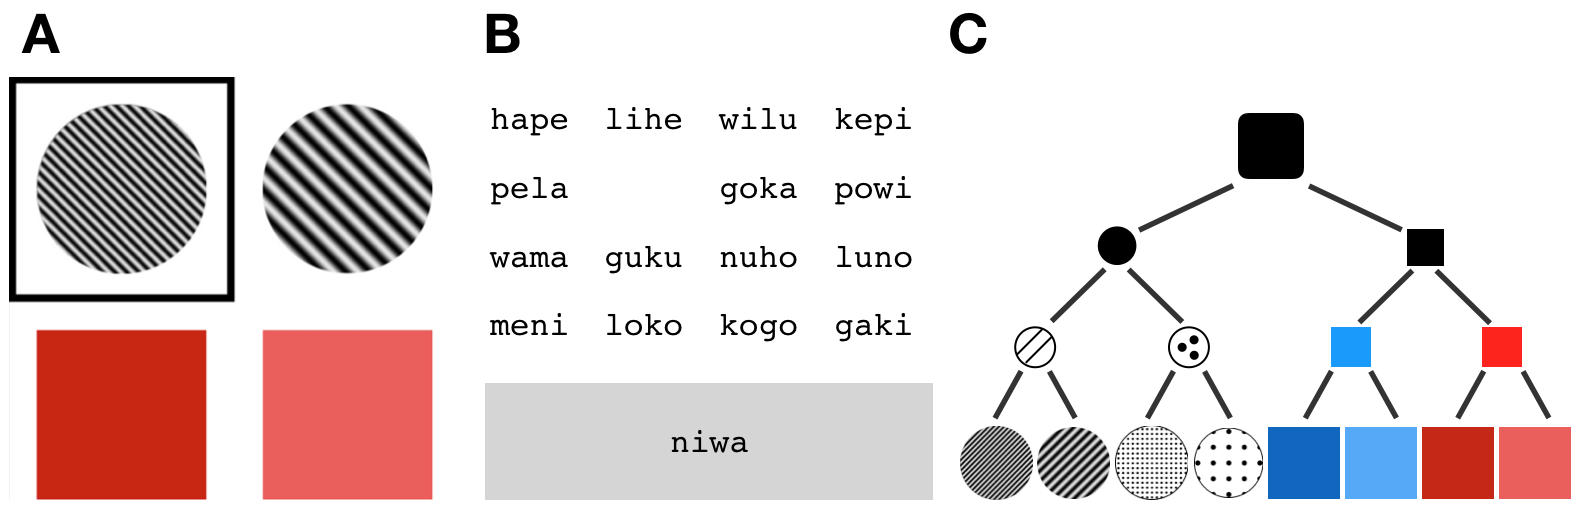
\includegraphics[scale=.6]{fig.png}}
{\caption{{(A) Example of \emph{fine} context where one of the distractors belongs to the same fine-grained branch of the hierarchy as the target (i.e.\ another striped circle), so any abstract label would be insufficient to disambiguate them. The target is highlighted for the speaker with a black square. (B) Drag-and-drop chat box interface. (C) Hierarchical organization of stimuli.\label{exp}}}}
\vspace{-2ex}
\end{center}
\end{figure*}

Here, we develop an experimental paradigm and analytic approach to examine the causal factors driving the emergence of lexical conventions in real-time. 
We manipulated context in a repeated reference game where pairs of participants interactively coordinated on an artificial language from scratch. %\cite<e.g.>{GalantucciGarrod11_ExperimentalSemiotics}.
%We manipulated the pragmatic demands of context and found that abstractions only emerged when  that for the optimal expressivity hypothesis in the lexica different pairs converged on, we conducted a Bayesian Data Analysis of a rational communication model to infer the underlying lexica participants were using throughout the game. 
Even though a complete communication system containing a distinct word for each object is feasible and sufficient for all contexts, we find that abstractions begin to emerge when fine-grained distinctions are not necessary. %We close with a discussion of learning mechanisms that may give rise to these dynamics.

%\ndg{this paragraph is too vague yet technical. either be more specific about design and results. or describe at the level of take-aways.}
% rational communication model allowing us to analyze not just what system they converged on but how it got there. % present a learning mechanism at the level of individual agents 
%Here, we show how the statistics of the communicative environment shape which levels of abstraction are lexicalized by interacting agents. 


% Repeated reference games 
%In this paper, however, . If there are multiple rabbits around, the travelers may need a specific conventionalized term for each; otherwise, they can achieve the same communicative success with fewer words by learning generalizations. When the pragmatics of the context allow for ambiguity in the intended level of reference, adaptive speakers can get away with extending the term more broadly. 


%% Example that sets up our specific hypothesis?

%Suppose, mixing thought experiments from \citeA{Wittgenstein09_PhilosophicalInvestigations} and \citeA{Quine13_WordAndObject}, that two travelers meet in a forest, with no language in common. One is cooking dinner, and the other agrees to help in exchange for food and shelter. What kind of micro-language do they coordinate on to solve this joint task, and how is it shaped by context? 
%To test intuitions about how pragmatics and context might affect the communication system they develop, we consider two cases. If there are multiple rabbits around, the travelers may need a specific conventionalized term for each; otherwise, they can achieve the same communicative success with fewer words by learning generalizations. 
			
\section{Experiment: Repeated reference game}

\subsubsection{Participants}

We recruited 278 participants from Amazon Mechanical Turk to play an interactive, multi-player game using the framework described in \citeA{Hawkins15_RealTimeWebExperiments}. Pairs were randomly assigned to one of three different conditions, yielding between $n=36$ and $n=53$ dyads per condition, after excluding participants who disconnected before completion.\footnote{All materials and data are available at \url{https://github.com/hawkrobe/conventionalizing_hierarchies}; planned sample sizes, exclusion criteria, and behavioral analysis plan were pre-registered at \url{https://osf.io/2hkjc/}.}

\subsubsection{Procedure \& Stimuli}
Participants were paired over the web and placed in a shared environment containing an array of objects (Fig.\ 1A) and a `chatbox' to send messages from a randomly generated vocabulary (Fig.\ 1B). On each of 96 trials, one player (the `speaker') was privately shown a highlighted target object and allowed to send a single word to communicate the identity of this object to their partner (the `listener'), who subsequently made a selection from the array. Players were given full feedback, swapped roles each trial, and both received bonus payment for each correct response.

The objects that served as referents were designed to cluster in a fixed three-level hierarchy with shape at the top-most level, color/texture at the intermediate levels, and frequency/intensity at the finest levels (see Fig.\ 1C). Each communicative context contained four objects. Distractors could differ from the target at various level of the hierarchy, creating different types of contexts defined by the finest distinction that had to be drawn. We focus on two: \emph{fine} trials, where the closest distractor belongs to the same fine-grained subordinate category (e.g.\ another striped circle; see Fig.\ 1A), and \emph{coarse} trials, where the closest distractor belongs to a coarser level of the conceptual hierarchy (e.g.\ dotted circle instead of striped circle).\footnote{Even coarser trials with super-ordinate distractors (e.g.\ a circle target among three square distractors) were logically possible but would have introduced several experimental confounds; we opted to leave these trial types out of our design and conduct the minimal manipulation.} Fixed arrays of 16 utterances (enough to allow the potential for full expressibility) were randomly generated for each pair (and held constant across trials) by stringing together consonant-vowel pairs into pronounceable 2-syllable words (see Fig.\ 1B).

Critically, we manipulated the statistics of the context in a between-subjects design to test the effect of communicative relevance on lexicalization. In the pure \emph{fine} and \emph{coarse} conditions, all targets appeared in fine or coarse contexts, respectively; in the \emph{mixed} condition, the two context types were equally likely%, providing diversity in the relevant distinctions that must be drawn. 
Sequences of trials were constructed by randomly shuffling targets and trial types within blocks and ensuring no target appeared more than once in a row. 

In addition to behavioral responses collected over the course of the game, we designed a post-test to explicitly probe players' final lexica. For all sixteen words, we asked players to select all objects that a word can refer to (if any), and for each object, we asked players to select all words that can refer to it (if any). Using a bidirectional measure allows us to check the internal validity of the lexica reported.%, to compare lexica across partners, and to distinguish between specific terms that apply to only one object and abstract terms that apply to all objects underneath higher nodes in the hierarchy. 

\subsection{Results}

\subsubsection{Partners successfully learn to communicate}

Although participants in all conditions began with no common basis for label meanings, performing near chance on the first trial (proportion correct $= 0.19$, 95\%~CI~$=~[0.13, 0.27]$), most pairs were nonetheless able to coordinate on a successful communication system over repeated interaction (see Fig.\ \ref{fig:accuracy}). 
A mixed-effects logistic regression on listener responses with trial number as a fixed effect, and including by-pair random slopes and intercepts, showed a significant improvement in accuracy overall, $z = 14.4, p < 0.001$. 
Accuracy also differed significantly \emph{across} conditions (Fig.\ \ref{fig:accuracy}): adding an additional main effect of condition to our logistic model provided a significantly better fit, $\chi^2(2) = 10.8, p = 0.004$. 
Qualitatively, the \emph{coarse} condition was easiest for participants, the \emph{fine} condition was hardest, and the \emph{mixed} condition was roughly in between. % Looking more closely at games within the mixed condition, we found that performance on subordinate and intermediate trial types roughly mirrored the gap between the .
Finally, the (log) response time taken by the speaker to choose an utterance also decreased significantly over the course of the game, $t = -19.7, p < 0.001$, indicating that lexical mappings became increasingly established or accessible.

\begin{figure}[t]
\begin{center}
{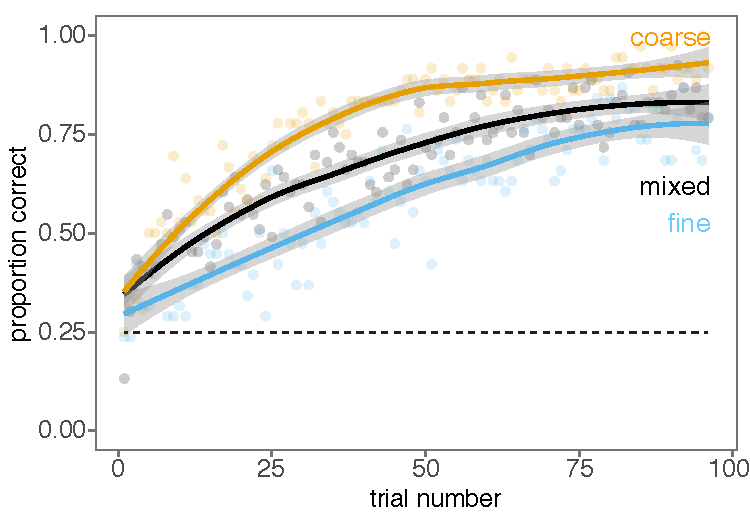
\includegraphics[scale=0.63]{accuracyByCondition_edited.pdf}}
%{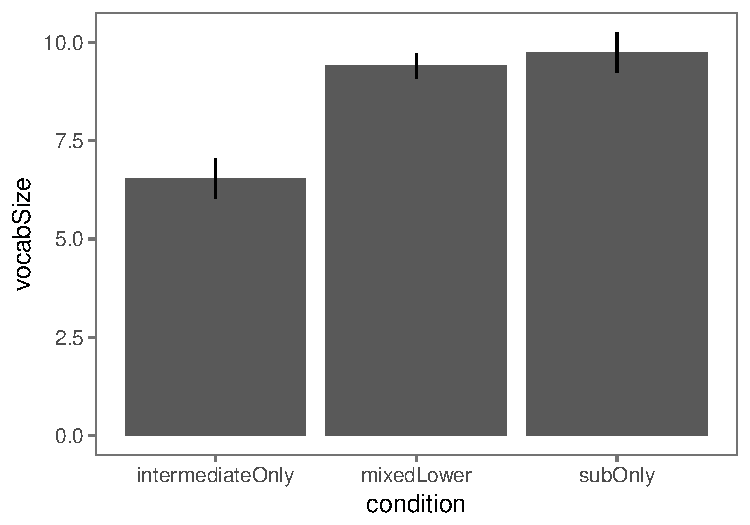
\includegraphics[scale=.64]{lexiconSize.pdf}}
\vspace{-2ex}
{\caption{{Players learn to coordinate on a successful communication system. Each point is the mean proportion of correct responses by listeners; curves are nonparametric fits.  %\todo[inline]{rdh questions: Use semantically meaningful condition codes, e.g.\ red/blue/purple? Is this too far aggregated from data (e.g.\ show error bars on each point? fit curves to individual-level binary responses instead of through group means?)}  
\label{fig:accuracy}}}}
\vspace{-3ex}
\end{center}
\end{figure}

\subsubsection{Partners converge on similar lexica}

Another indicator of successful learning is convergence or alignment of lexica across partners in a dyad. Before using post-test responses to compute similarity \emph{across} partners, however, we examine the internal consistency \emph{within} an individual's post-test responses. For each participant, we counted the number of mismatches between the two directions of the lexicon question (e.g.\ if they clicked the word `mawa' when we showed them one of the blue squares, but failed to click that same blue square when we showed `mawa'). In general, participants were quite consistent: out of 128 cells in the lexicon matrix (16 words $\times$ 8 objects), the median number of mismatches was 2 (98\% agreement), though the distribution has a long tail (mean $= 7.3$). We therefore conservatively take a participant's final lexicon to be the \emph{intersection} of their word-to-object and object-to-word responses.

Using these estimates of each participant's lexicon, we compute the overlap between partners. For most pairs, partners aligned strongly by the end, with a median post-test overlap of 97.6\% (125 out of 128 entries). Because these matrices were extremely sparse, however, just a a few mismatches could have a large impact on performance. Overall accuracy in the game is strongly correlated with alignment: partners who reported more similar lexica at the end tended to perform better at the task ($r = 0.77$).  

Despite these markers of success at the group level, individual performance was bimodal: a subpopulation of 29 games (11\% of coarse games, 18\% of mixed, and 39\% of fine) still showed relatively poor performance, sometimes at chance, by the end of the game. For the subsequent analyses focusing on the content of the lexicon, we exclude games with fourth-quartile accuracy below the pre-registered criterion of 75\% to ensure we are examining only successful lexica. %After removing these participants, internal consistency was roughly similar across conditions (means of 3.0 and 3.4 internal mismatches in the \emph{coarse} and \emph{fine} conditions, and 5.8 in \emph{mixed}) so we don't expect these to bias our data.

\subsubsection{Contextual pressures shape the lexicon}

We predicted that in contexts regularly requiring speakers to make fine distinctions among objects at subordinate levels of the hierarchy, we would find lexicalization of specific terms for each object (indeed, a one-to-one mapping may be the most obvious solution in a task with only 8 objects). Conversely, when no such distinctions were required, we expected participants to adaptively lexicalize more abstract terms. One coarse signature of this prediction lies in the \emph{efficiency} of the resulting lexicon: lexicalizing abstract terms should require participants to use fewer terms overall.

To test this prediction, we counted the number of words in each participant's reported lexicon (i.e.\ the words for which they marked at least one object in the post-test). We found that participants in the \emph{coarse} condition reported significantly smaller, more efficient lexica ($m = 4.9$ words) than participants in the \emph{mixed} and \emph{fine} conditions ($m = 7.4, t = 10.3, p <0.001$ and $m = 7.6, t = 9.5, p < 0.001$, respectively; see Fig.\ \ref{fig:lexiconContent}A). At the same time, the smaller lexicon provided equivalent coverage of objects: the median number of objects where participants agreed on the same word or words was 7, 6.5, and 7, respectively. 

\begin{figure*}[t]
\begin{center}
{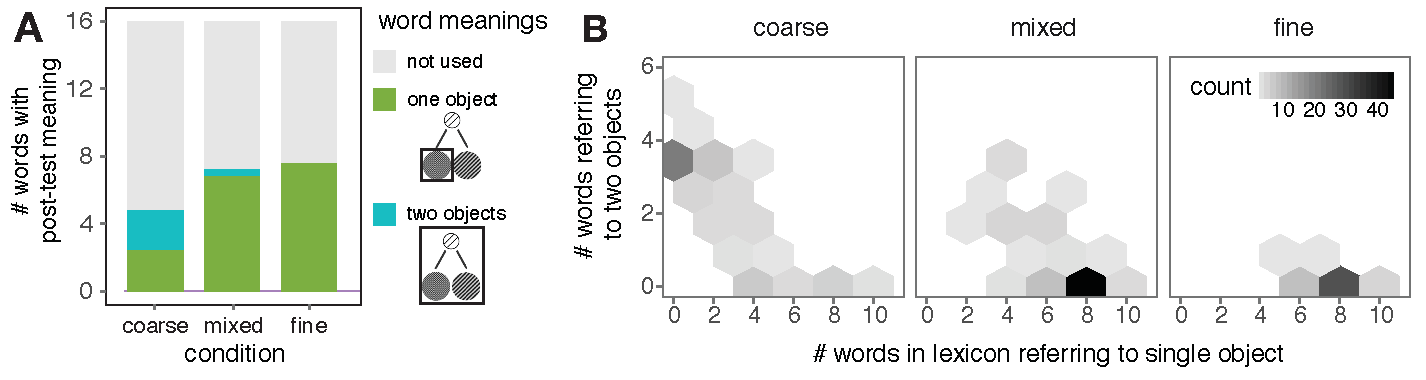
\includegraphics[scale=0.73]{resultsFig_v1.pdf}}
\vspace{-2ex}
{\caption{{Pragmatic demands of context shape the formation of abstractions. (A) Mean number of words participants reported with specific meanings (applying to 1 object) or abstract meanings (applying to 2 objects).
%Each participant provided meanings for all sixteen words in their vocabulary box (including selecting no objects if it had no meaning). 
%In the \emph{coarse} condition, participants reported fewer total words in their vocabulary and more of the words they did have were abstractions applying to more than one object. %Distribution of extension sizes in lexica reported across conditions, including those with no extensions  
%\todo[inline]{KS: You'll have to explain how a word can have no extensions, but I'd be tempted to not show these in these graphs? Assuming these are uninteresting (?), showing proportion of  1 vs more-than-1 object words would make the result much clearer. Do you have this in to also show the lexicon size difference? Could show that more straightforwardly with a plot of number of words poer condition?} . 
%Nearly every word reported in the \emph{fine} condition referred to a single object and the \emph{mixed} condition is more similar to the \emph{fine} condition than the \emph{coarse} condition.
(B) Diversity of terms within reported lexica: many participants in the \emph{coarse} condition reported a mixture of abstract and specific terms.% \todo[inline]{TODO: A/B labels; use \# words instead of \%; change axis labels in B to `'' and ``\# words referring to multiple objects'';}  
\label{fig:lexiconContent}}}}
\end{center}
\vspace{-2ex}
\end{figure*}

If participants in the \emph{coarse} condition can get away with fewer words in their lexicon, what are the meanings of the words they do have? We counted the numbers of `specific' terms (e.g.\ words that refer to only one object) and `abstract' terms (e.g.\ words that refer to two objects) in the post-test. We found that the likelihood of lexicalizing abstractions differed systematically across conditions (see Fig.\ \ref{fig:lexiconContent}A). Participants in the \emph{fine} condition reported lexica containing exclusively specific terms, while participants in the \emph{coarse} condition reported significantly more abstract terms ($m = 2.5, p < 0.001$). 

These data also reveal an interesting asymmetry in lexicon content across conditions: while abstractions are entirely absent from the \emph{fine} condition, participants in the other conditions often reported a mixture of terms (see Fig.\ \ref{fig:lexiconContent}B). In the \emph{coarse} condition, for instance, participants could in principle perform optimally with only four abstract terms and no specific terms. While this was the modal system that emerged (reported in the post-test by nearly 1/3 of participants), the average proportion of abstract (vs.\ specific) terms \emph{within} each participant's lexicon in the \emph{coarse} condition ($m = 0.56$) was significantly higher than in the other conditions ($p < 0.001$, exploratory).
%\ndg{`average entropy of the distribution of abstract vs.\ specific terms within each participant's lexicon' is a lot to swallow at once...}

\section{Model-based Analysis}

Our post-test provides some insight into the end-result of lexicalization under different communicative contexts, but understanding the \emph{dynamics} of lexicalization requires a more detailed analysis of behavioral trajectories. How do lexica shift and develop over the course of interaction? 

In this section, we present a statistical model of this progression. We assume that on any given trial, speakers and listeners are rationally producing and interpreting utterances given some internal lexicon, and we use a Bayesian statistical model to infer their lexicon from their behavior. First, this analysis validates our post-test measures of lexical meaning against actual behavioral usage --- if participant reports are internally consistent, the model's posterior near the end of the game should predict their post-test responses. Second, we can examine the time-course of lexical emergence by inspecting lexica inferred from early behavior in the game. %We expect this latter to be more broadly useful in studies where explicit measurements of the lexicon are not practical. %Finally, because our statistical model learns from the same data that agents in principle learn from, it provides some insight into the path-dependent effects of early communicative pressures on the available meanings. %basic-level vs.\ subordinate-level terms, (4) measure path-dependence, e.g.\ how 


\subsection{Generative model}

We begin with a generative model of how agents use their underlying lexicon to produce and interpret language. This model provides a linking function assigning a likelihood to the speaker utterances and listener choices we observe on each trial, given any latent lexicon. We adopt the probabilistic Rational Speech Act (RSA) framework, which has been successful in recent years at capturing a broad array of pragmatic phenomena in language use \cite{GoodmanFrank16_RSATiCS,FrankeJager16_ProbabilisticPragmatics}. This framework captures the Gricean assumption of cooperativity: a pragmatic speaker $S_1$ attempts to be informative in context while a pragmatic listener $L_1$ inverts their model of the speaker to infer the intended target. The chain of recursive social reasoning grounds out in a \emph{literal listener} $L_0$, which directly soft-maximizes its lexicon, $\mathcal{L}^t(w,o)$, to interpret a given utterance. This model can be formally specified as follows:
$$
\begin{array}{rcl}
L_0(o_i | w, \mathcal{L}^t) &\propto  & \exp\{\mathcal{L}^t(w,o_i)\} \\
S_1(w | o_i, \mathcal{L}^t) &\propto & \exp\{\ln L_0(o_i | w, \mathcal{L}^t)\} \\
L_1(o_i | w, \mathcal{L}^t) &\propto  & S_1(w | o_i, \mathcal{L}^t) P(o_i) 
\end{array}
$$
% MF: adjusted this for better vertical spacing wrt adjacent paragraphs
where $o_i$ is a chosen object and $w$ an uttered word.

We use these pragmatic speaker and listener likelihood functions to link latent lexica, represented as a matrix of real values $\ell_{w,o}^t \in \mathbb{R}$, to behavior.
%<<<<<<< HEAD
%This allows us to then use Bayesian inference to back out the effective lexicon from trial-by-trial behavior.
%Because each trial has only a single choice, we share statistical strength within periods of time by using a quartile-wise hierarchical prior. 
%In particular, we assume that each lexicon entry on round $t$ is drawn from a Gaussian $\mathcal{N}(m^{q}_{w,o}, \sigma)$ centered at that quartile's hyper-lexicon with some fixed dispersion, and mapped to the unit interval with a logistic function\footnote{The logistic function is given by $\text{logistic}(x) = 1/(1 + e^{x})$.}:
%$$
%\begin{array}{rcl}
%m_{w,o}^q &\sim& \mathcal{N}(0, 1)\\
%\sigma &\sim& \text{abs}(\mathcal{N}(0, 0.5)) \ndg{fixme} \\ 
%m_{w,o}^t &\sim& \mathcal{N}(m_{w,o}^q,  \sigma)\\
%\ell_{w,o}^t &=& \text{logistic}(m_{w,o}^t)
%\end{array}
%$$
%
%We approximate the posterior of this model using mean-field variational inference \cite{RanganathGerrishBlei13_BlackBoxVariationalInference}, implemented in the probabilistic programming language WebPPL \cite{GoodmanStuhlmuller14_DIPPL,DAIPP}. 
%The approximating family for each random variable is Gaussian \ndg{really? even for bounded ones like $\alpha$?}.
%This approximates the joint posterior over all lexical entries (and shared hyperparameters) used by each participant for each round in each game. 
%\ndg{there are two hyperparameters, $\alpha$ and $\sigma$, right? need to say what prior we use for them. these are shared across quartiles, trials, and participants, or separately?}
%=======
This allows us to then use Bayesian inference to back out each participant's effective lexicon from their trial-by-trial behavior.
Because each trial has only a single choice for each player, we pool statistics within $k$ epochs of the data (we choose $k=6$ such that each target appears exactly twice in each epoch). 
For each epoch, we sample lexical entries from independent Gaussian priors: $$\ell_{o,w}^k\sim\mathcal{N}(0, 5)$$ This prior is intended to regularize lexicon entries to be relatively close to 0, inducing a bias toward sparsity. %centered at that epoch's hyper-lexicon with some fixed dispersion, and mapped to the unit interval with a logistic function:%\footnote{The logistic function is given by $\text{logistic}(x) = 1/(1 + e^{x})$.}:
%\begin{alignat*}{3}
%& \sigma & \sim & \textrm{abs}(\mathcal{N}(0, 0.5)) \\
%& \ell_{w,o}^k &\sim& \mathcal{N}(0, 3)\\
%& m_{w,o}^t &\sim& \mathcal{N}(m_{w,o}^k,  \sigma)\\
%& \ell_{w,o}^t &=& \text{logistic}(m_{w,o}^t)
%\end{alignat*}

We approximate the posterior of this model separately for each pair using mean-field variational inference, implemented in the probabilistic programming language WebPPL \cite{GoodmanStuhlmuller14_DIPPL,DAIPP}. 
The approximating family for each random variable is Gaussian. We approximate the joint posterior over all lexical entries used in each epoch by each participant. 


\begin{figure*}[t]
\begin{center}
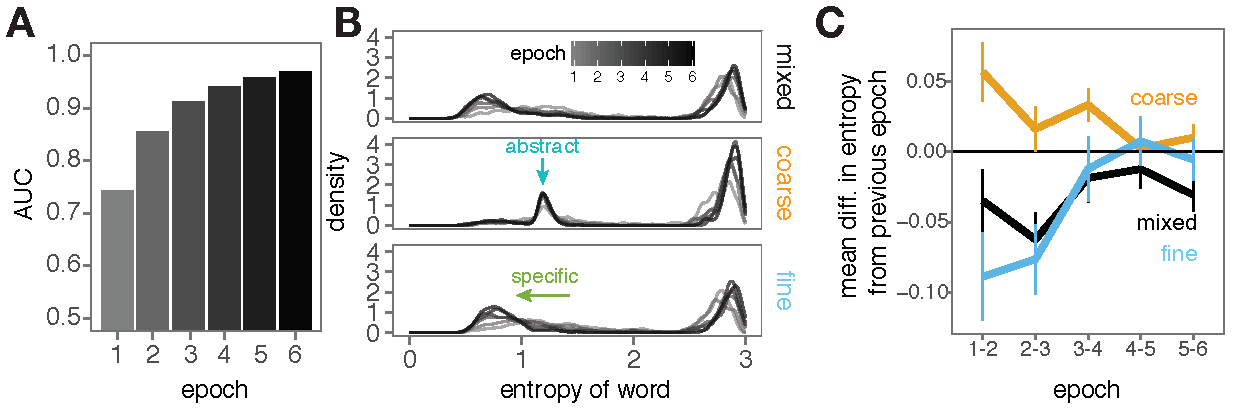
\includegraphics[scale=0.84]{modelFig.pdf}
\vspace{-1ex}
{\caption{{Model-based results. (A) A logistic classifier based on inferred lexical entries accurately predicts post-test responses. (B) Entropy of posterior word extensions show coalescence across epochs for each condition. (C) Mean change in entropy at the word level from trial to trial (error bars are $\pm 1$ SE)}  \label{fig:postTestPrediction}}}
\end{center}
\vspace{-3ex}
\end{figure*}

% We place a relatively uninformative but regularizing prior $\ell_{w,o}^0 \sim \mathcal{N}(0, 1)$ on the entries of the quartile-level lexica. 
%\ndg{this paragraph can be simplified. it will help to give statistician's notation block defining model. if each lexical entry is treated independently, then just do at that level.... something like:}

%We capture the temporal dependence of subsequent lexica by placing a Gaussian random walk on lexical entries: the lexicon at time $t+1$ is sampled from a Gaussian distribution centered at the lexicon on the previous trial: $$\ell_{w,o}^{t+1} \sim \mathcal{N}(\ell_{w,o}^t, \sigma)$$ where sigma is a hyperparameter determining the drift rate. \todo[inline]{Is this related to the bayesian RL thing in Mathys et al, 2011?}
%\ndg{collect the RSA eqs into one block, with a paragraph of description. don't need much.}

%\todo[inline]{TODO: Be explicit about how this allows us to strengthen our inferences? Needs to be cleaned up.}
%This allows us to learn about meanings of words and objects we haven't seen. e.g.\ suppose we hear a speaker say `mimi' to refer to one of the blue squares in the context of the other blue square. If `mimi` applied to both blue squares equally well in their lexicon, then the data would be extremely unlikely: the speaker would have avoided such an underinformative utterance. The data is much more likely under a lexicon where `mimi` only refers to the target blue square much more strongly.  Similarly, if another word in their lexicon was more informative in distinguishing these items, we assume they would have used it. Note that when the same utterance is used in a coarse trial, where only one of the blue squares is in context, it is ambiguous whether or not it can also apply to the other blue square.

%RSA provides a linking function from $\mathcal{L}^t$ to speaker and listener behavior, which is differentiable with respect to the lexica.
%We use mean-field variational inference \cite{RanganathGerrishBlei13_BlackBoxVariationalInference}, implemented in the probabilistic programming language WebPPL \cite{GoodmanStuhlmuller14_DIPPL}. We optimize a family of Gaussians to minimize the evidence lower bound (ELBO) which approximates the joint posterior over all lexical entries (and shared hyperparameters) used by each participant for each round in each game. 

%\begin{figure}[t]
%\begin{center}
%{\includegraphics[scale=.4]{modelSchematic}}
%%{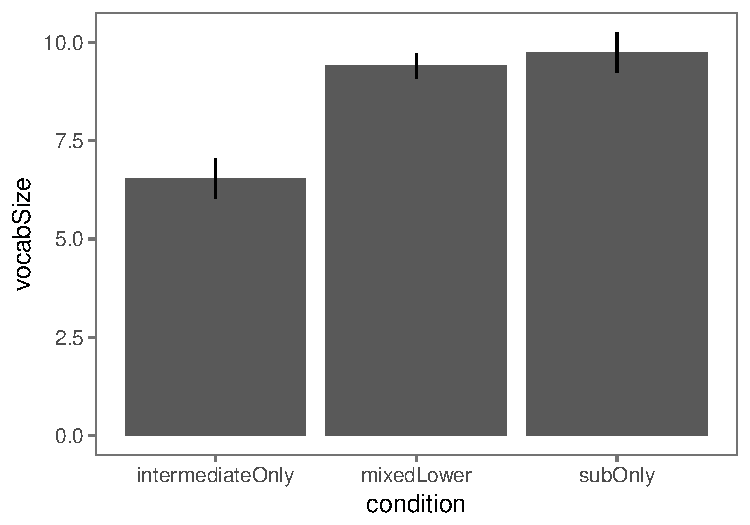
\includegraphics[scale=.64]{lexiconSize.pdf}}
%{\caption{{\footnotesize \todo[inline]{question for NDG: I wanted some kind of schematic of the model, but I'm not sure this plate notation is the best way of doing it (whether supplementing plate with a cartoon, or replacing it?)\dots Notation is kind of icky right now, too\dots this would ideally lay out very clearly the intuition behind how early contexts affect lexicon learning}  \ndg{i'd cut this. i don't think you need a bda model figure.}   \label{fig:modelSchematic}}}}
%\end{center}
%\end{figure}

\subsection{Validating post-test responses}

We begin by showing that the lexical entries we infer for each participant accurately predict their post-test responses. 
We constructed a logistic classifier from our posterior on each epoch: for each object-word pair $(o,w)$ in the post-test response matrix, we computed the marginal posterior probability $P(\ell_{o,w} > 0.5| \theta_{o,w})$, where $\theta_{o,w}$ are the corresponding variational parameters (i.e. the mean and variance of the approximating Gaussian). This gives the posterior probability that word $w$ applies to object $o$. We evaluated the performance of this classifier by constructing an ROC curve that shows the tradeoff between hits and false alarms as the discrimination criterion is varied. We found that the classifier based on the final epoch predicts post-test responses with excellent accuracy (AUC: $0.98$; see Fig.\ \ref{fig:postTestPrediction}A). This indicates that the post-test lexicon is indeed linked to behavior as predicted by RSA, validating both the post-test measure and the results of our Bayesian analysis.

Furthermore, we found that the corresponding posterior predictives from earlier epochs predicted final post-test responses less well, even though they were learned from the same number and type of behavioral observations (Fig.\ \ref{fig:postTestPrediction}A). Still, even the classifier based on the earliest epoch performs above chance, indicating that some information about the final lexicon is available from the earliest trials. These patterns are suggestive of a path-dependent process where the lexicon gradually coalesces from initially arbitrary associations over the course of interaction. We next turn to the earliest stages of this process.% to examine this process in more detail.

\subsection{Examining early time course}

%\todo[inline]{note for MF: I got this feature-based model working and then Noah thought it might be better to just use the simple model for everything? I'm going to see how far I can run with the simple model, so this section is somewhat in flux\dots}

%Classic theories in historical linguistics distinguish between semantic \emph{broadening}, when a word takes on a more inclusive meaning, and \emph{narrowing}, when meanings become more restrictive over time \cite{TraugottDasher02_RegularitySemanticChange}. 
One advantage of the statistical approach we develop here is the ability to make descriptive inferences about the meanings being used in settings where we \emph{don't} ask participants for explicit judgements---in particular, in early trials of our games. 

Our primary measure of interest is the \emph{entropy} of the extension of words over the eight objects. The entropy of a particular word is near zero when its meaning is peaked on a single object, and is maximized when could apply equally to all objects (e.g. for a novel word that has not yet been used). 
%In principle, we would find uniform distributions for words that apply equally well to all eight objects, but in our case, uniform meanings are more likely to reflect the uncertainty in our model's posterior (e.g. for words that were never used in a game). 
We expect abstract terms to lie in between these extremes. 
We obtain the extension distribution for each word by running it through our $L_0$ model, essentially asking how likely it is to refer to each of the eight objects.\footnote{Using $L_0$, rather than $L_1$ or $\mathcal{L}$, gives us a notion of word extension that is close to the underlying lexicon while influenced by non-identifiability of parameters. For instance, $\mathcal{L}$ has an overall scaling per row that doesn't influence behavior.} 
We use the MAP estimate of the lexicon. % (in order to make entropy effects more evident). 
The resulting distribution of estimated word entropies, aggregated for each epoch and condition, is shown in Fig. \ref{fig:postTestPrediction}B. %There are two properties to note here. 
Abstract terms begin to form early (epoch 2) in the \emph{coarse} condition, and remain stable throughout the game. In contrast, specific terms are relatively slow-forming (epoch 4-5) in the other two conditions. The peak near an entropy of 3 reflects the inferred ambiguity of words that were not used or used randomly.

Because these distributions are aggregated across words, however, they leave open the possibility that lexica are not stabilizing or coalescing but simply cycling through different words each epoch. We address these dynamics more thoroughly at the \emph{word} level by computing the difference in each word's entropy from epoch to epoch (Fig. \ref{fig:postTestPrediction}C). For all conditions, we found that the entropy of individual words changed less over later epochs (i.e. the difference scores approached zero), indicating that meanings gradually stabilized. There are also differences across conditions: words in the \emph{mixed} and \emph{fine} condition began with high entropy reduction (becoming more specific) which continued through the final epochs, while words in the \emph{coarse} condition actually seemed to increase in entropy across the game on average. %(as the set of completely unused words grew \ndg{do we know this is why?}) 
%while words in the other conditions decrease their entropy. 
%(as unused words were increasingly recruited to fulfill the demand for specific names
%\ndg{again do we know that it's this?}

These preliminary results, then, may reflect a combination of narrowing and broadening depending on condition. Unknown words can initially refer to any of the objects and only acquire more informative meanings as agents learn through interaction. Yet in the coarse condition where agents are quick to adopt meanings, the rest of the game may be spent paring down the lexicon instead.

%\ndg{i think we should try to squeeze in a figure for the entropy differences...}

%For this analysis, we elaborated our model to use an underlying feature basis to derive the lexicon instead of independent entries for each object-word combination. 
%\ndg{can't we first do this analysis using the simple lexicon model? }
%That is, we re-encoded each of the eight objects as a point in a discrete seven-dimensional feature space roughly corresponding to the nodes of the hierarchy\footnote{(shape, red-ness, blue-ness, stripe-ness, spot-ness, pattern frequency, and color intensity)} and learned an embedding for each word in this space. The meaning function used by our literal listener, then, is simply $L^2$ similarity between the word and object vectors. This feature-based representation has two useful properties. First, it allows for more meaningful feature-based generalization: having observed a word associated with one red square, it is more likely to extend this term to the other red square than to a striped circle simply because of their relative distances in the space. Second, it provides a way to directly read out more abstracted terms from the inferred lexicon (e.g.\ by looking at whether the red-ness feature is high and the brightness term is at the mid-point). 

%The mixed pairs can get by with their lexicon of specific terms, and even the coarse pairs are stuck with the residue of their early specific terms. 

%\todo[inline]{TODO: use simple model to look at the expected extension size of each word, and how it changes between quartiles.... walk through examples of early rounds in different contexts; show timecourse of abstractions, e.g.\ are initially specific terms extended or are initially abstract terms narrowed?  Do you tend to move from big to small or small to big quarter-to-quarter?}

\section{Discussion}

How and why do abstractions emerge in local interactions? We hypothesized that although communicative contexts requiring fine distinctions would favor one-to-one object-word mappings, pressures for efficiency would allow abstractions to emerge in coarser contexts. By manipulating context statistics in a real-time experiment, we found evidence for these pragmatic influences on interactive convention formation.

Our results may help to illuminate the relationship between our concepts and words, which are often treated interchangeably. While our mental taxonomies are adaptive to the natural perceptual structure of the world \cite{MervisRosch81_CategorizationReview} %(Rosch et al, 1976; Mervis \& Rosch ,1981; Murphy \& Smith, 1982), 
it is far from inevitable that all levels of these conceptual hierarchies become conventionalized as lexical items. There are many perfectly natural concepts that are not represented by distinct words in the English language: for instance, we do not have words for each tree in our yards, or for ad-hoc concepts %like \emph{things to sell at a garage sale} 
\cite{Barsalou83_AdHocCategories}. Indeed, English speakers are often fascinated by foreign words like the Danish ``hygge'' (a specific notion of coziness) or Scottish ``tartle'' (hesitating when introducing someone because you've forgotten their name) that are difficult to express in English.
Our results highlight communicative needs to distinguish, in context, as a force behind the choice to lexicalize some fine-grained concepts. 
A related direction for future work is to explore the relationship between communicative need and \emph{basic-level} structure.

While we showed how abstract words emerge from efficiency even in a task requiring only reference to individual objects, there are other clear functional advantages to having abstract terms in the lexicon. For one, they allow speakers to efficiently refer to large, potentially infinite, sets of things, and make generalizations about categories, e.g.\ ``Dogs bark'' \cite{TesslerGoodman16_Generics}. Future work should explore this as an additional pressure toward abstract, nested nouns.
Similarly, the option to refer to more specific concepts with compound terms (e.g.~``spotted dog''), which was not available in our experiment, may impact final conventions.
We expect that labels will become lexicalized when the cost incurred by frequently using a compositional construction exceeds the cost of adding an additional word to the lexicon. 
Future work should also explore these hypotheses about how lexicalization of nominal terms trades off with compositionality. 


%\todo[inline]{question for NDG: Should we comment on some methodlogical things people put in the `strategy' box? e.g.\ some people seem to be taking notes or using sound-symbolic associations like "nogo" to mean "red" (not a problem; should just help memory or help make initial meanings not entirely arbitrary but shouldn't change contextual demands\dots)}

%\todo[inline]{question for MF: put some broader comment connecting to/contrasting with other cognitive theories of what's going on here? e.g.\ (1) not a simple associative learning account, where people just store memory traces of word-object co-occurances (can't account for context effects of generation), although note that probably a simpler model just counting co-occurences could account for the post-test responses just as well (it just wouldn't have as flexible an underlying representation). (2) elaborates on Xu \& Tenenbaum (2007) word learning story by introducing contextual pressures?}
%\ndg{could do if there is a short clear point to make...}
%\mf{phew, not sure there is enough space and hesitant that this might wake sleeping dogs, no matter how careful we are}


Finally, although we implemented a purely statistical Bayesian data analysis model to infer lexica, it is also possible to consider a cognitive model of participants' own lexical inferences. Indeed, our findings are consistent with a recent cognitive model of convention formation which explained the rapid coordination on efficient but informative lexical terms as a process of mutual lexical learning \cite{HawkinsFrankGoodman17_ConventionFormation}. %Instead of simply using RSA as a linking function to analyze the snapshot meanings without assuming anything about how \emph{agents} might be learning or developing their lexica in response their partner -- . 
In this model, each agent assumes their partner is rationally producing cooperative utterances under some latent lexicon; given initial uncertainty over the contents of that lexicon, agents can invert their model of their partner to infer their lexicon from observable behavior. 
The different dynamics we observed across conditions, then, may be the consequence of different lexical inferences in different local contexts. Further, while we used RSA as a linking function in our statistical model, a cognitive model would allow us to test to what extent pragmatic reasoning is necessary to explain behavior.% may result from the different inferences made by pragmatic agents about the lexicon.  % \cite{BergenLevyGoodman16_LexicalUncertainty}. %Each individual is trying to infer the lexicon being used by their partner by observing their behavior in context. 

Our shared lexical conventions are richly structured systems with meanings at multiple levels of abstraction. There is now abundant evidence that languages adapt to the needs of their users, and the context-sensitive emergence of abstractions demonstrated in this paper suggests that the driver of this adaptation may lie in the remarkably rapid adaptability of agents themselves. We are constantly supplementing our existing language with local conventions as we need them. Our separate minds may organize the world into meaningful conceptual hierarchies but our shared language only evolves to reflect this structure when it is communicatively relevant. 



% For an example of a full page figure, see Fig.~\ref{fig:myFullPageFigure}.

